\documentclass[12pt,spanish,openany,letterpaper,pagesize]{scrbook}

\usepackage[utf8]{inputenc}
\usepackage[spanish]{babel}%escribir con acentos sin necesidad de comandos \'{} .
\usepackage{fancyhdr}
\usepackage{epsfig}
\usepackage{epic}
\usepackage{eepic}
\usepackage{amsmath}
\usepackage{amsfonts} 
\usepackage{amssymb}
\usepackage{threeparttable}
\usepackage{amscd}
\usepackage{here}
\usepackage{graphicx}
\usepackage{lscape}
\usepackage{blindtext}
\usepackage{hyperref}
\usepackage{tabularx}
%\usepackage{subfigure}
\usepackage{longtable}
\usepackage[square,numbers]{natbib}
\usepackage{caption}
\usepackage{subcaption}
\setcounter{tocdepth}{4}
\setcounter{secnumdepth}{2}

\usepackage{rotating} %Para rotar texto, objetos y tablas seite. No se ve en DVI solo en PS. Seite 328 Hundebuch
                        %se usa junto con \rotate, \sidewidestable ....


\renewcommand{\theequation}{\thechapter.\arabic{equation}}
\renewcommand{\thefigure}{\textbf{\thechapter.\arabic{figure}}}
\renewcommand{\thetable}{\textbf{\thechapter.\arabic{table}}}


\pagestyle{fancyplain}%\addtolength{\headwidth}{\marginparwidth}
\textheight22.5cm \topmargin0cm \textwidth16.5cm
\oddsidemargin0.5cm \evensidemargin-0.5cm%
\renewcommand{\chaptermark}[1]{\markboth{\thechapter\; #1}{}}
\renewcommand{\sectionmark}[1]{\markright{\thesection\; #1}}
\lhead[\fancyplain{}{\thepage}]{\fancyplain{}{\rightmark}}
\rhead[\fancyplain{}{\leftmark}]{\fancyplain{}{\thepage}}
\fancyfoot{}
\thispagestyle{fancy}%


\addtolength{\headwidth}{0cm}
\unitlength1mm %Define la unidad LE para Figuras
%\mathindent0cm %Define la distancia de las formulas al texto,  fleqn las descentra
\marginparwidth0cm
\parindent0cm %Define la distancia de la primera linea de un parrafo a la margen

%Para tablas,  redefine el backschlash en tablas donde se define la posici\'{o}n del texto en las
%casillas (con \centering \raggedright o \raggedleft)
\newcommand{\PreserveBackslash}[1]{\let\temp=\\#1\let\\=\temp}
\let\PBS=\PreserveBackslash

%Espacio entre lineas
\renewcommand{\baselinestretch}{1.1}

%Neuer Befehl f\"{u}r die Tabelle Eigenschaften der Aktivkohlen
\newcommand{\arr}[1]{\raisebox{1.5ex}[0cm][0cm]{#1}}

%Neue Kommandos
\usepackage{Befehle}
%Inicio del documento. Tener en cuenta que hay archivos auxiliares

\begin{document}
\pagenumbering{roman}
%\newpage
%\setcounter{page}{1}
\begin{center}
\begin{figure}
\centering%

\epsfig{file=HojaTitulo/EscudoUN,scale=1}%
\end{figure}
\thispagestyle{empty} \vspace*{2.0cm} \textbf{\huge
Agujero negro rotante en gravedad masiva dRGT}\\[6.0cm]
\Large\textbf{Jhon Sebastián Moreno Triana}\\[6.0cm]
\small Universidad Nacional de Colombia\\
Facultad de ciencias, Departamento de física\\
Bogotá, Colombia\\
2022\\
\end{center}

\newpage{\pagestyle{empty}\cleardoublepage}

\newpage
\begin{center}
\thispagestyle{empty} \vspace*{0cm} \textbf{\huge
Agujero negro rotante en gravedad masiva dRGT}\\[3.0cm]
\Large\textbf{Jhon Sebastián Moreno Triana}\\[3.0cm]
\small Trabajo de grado presentado como requisito parcial para optar al
t\'{\i}tulo de:\\
\textbf{Físico}\\[2.5cm]
Director:\\
Ph.D. en Fisica Eduard Alexis Larrañaga Rubio\\[2.0cm]

Agujeros negros en gravedad dRGT\\
Seminario de Agujeros negros\\[2.5cm]
Universidad Nacional de Colombia\\
Facultad de ciencias, Departamento de Física\\
Bogotá, Colombia\\
2022\\
\end{center}

\newpage{\pagestyle{empty}\cleardoublepage}

\newpage
\thispagestyle{empty} \textbf{}\normalsize
\\\\\\%
\textbf{(Dedicatoria o un lema)}\\[4.0cm]

\begin{flushright}
\begin{minipage}{8cm}
    \noindent
        \small
        
\end{minipage}
\end{flushright}

\newpage{\pagestyle{empty}\cleardoublepage}

\newpage
\thispagestyle{empty} \textbf{}\normalsize
\\\\\\%
\textbf{\LARGE Agradecimientos}
\addcontentsline{toc}{chapter}{\numberline{}Agradecimientos}\\\\


\newpage{\pagestyle{empty}\cleardoublepage}

\newpage
\textbf{\LARGE Resumen}
\addcontentsline{toc}{chapter}{\numberline{}Resumen}\\\\
\\[2.0cm]

\textbf{\small Palabras clave: }\\


\textbf{\LARGE Abstract}\\\\
\\[2.0cm]
\textbf{\small Keywords: }\\

\renewcommand{\tablename}{\textbf{Tabla}}
\renewcommand{\figurename}{\textbf{Figura}}
\renewcommand{\listtablename}{Lista de Tablas}
\renewcommand{\listfigurename}{Lista de Figuras}
\renewcommand{\contentsname}{Contenido}


%\newcommand{\clearemptydoublepage}{\newpage{\pagestyle{empty}\cleardoublepage}}
\cleardoublepage
 % para que aparezca en el indice de contenidos
\tableofcontents


%\cleardoublepage
%\addcontentsline{toc}{chapter}{Lista de figuras} % para que aparezca en el indice de contenidos
%\listoffigures % indice de figuras



%\chapter*{Lista de s\'{\i}mbolos}
\addcontentsline{toc}{chapter}{\numberline{}Lista de s\'{\i}mbolos}
Esta secci\'{o}n es opcional, dado que existen disciplinas que no manejan s\'{\i}mbolos y/o abreviaturas.\\

Se incluyen s\'{\i}mbolos generales (con letras latinas y griegas), sub\'{\i}ndices, super\'{\i}ndices y abreviaturas (incluir s\'{o}lo las clases de s\'{\i}mbolos que se utilicen). Cada una de estas listas debe estar ubicada en orden alfab\'{e}tico de acuerdo con la primera letra del s\'{\i}mbolo.
\section*{S\'{\i}mbolos con letras latinas}
 \label{simbolos}
 \renewcommand{\arraystretch}{1.3}
%\begin{longtable}[l]{*{4}{>{$}l<{$}}p{9cm}}
\begin{longtable}[l]{>{$}l<{$}l>{$}l<{$}>{$}l<{$}}
%\begin{tabular}
\textbf{S\'{\i}mbolo}&\textbf{T\'{e}rmino}&\textbf{Unidad SI}&\textbf{Definici\'{o}n}\\[0.5ex]\hline
\endfirsthead%
\textbf{S\'{\i}mbolo}&\textbf{T\'{e}rmino}&\textbf{Unidad SI}&\textbf{Definici\'{o}n}\\[0.5ex]\hline
\endhead%
      A              &\'{A}rea                                   &\text{m}^{2}                         &\int\int dxdy\\%
      A_{\text{BET}} &\'{A}rea interna del s\'{o}lido                &\frac{\text{m}^{2}}{\text{g}}        &\text{ver DIN ISO 9277}\\%
      A_{\text{g}}   &\'{A}rea transversal de la fase gaseosa    &\text{m}^{2}                         &\text{Ec...}\\%
      A_{\text{s}}   &\'{A}rea transversal de la carga a granel  &\text{m}^{2}                         &\text{Ec...}\\%
      a              &Coeficiente                            &1                                    &\text{Ec...}\\%
      a              &Contenido de ceniza                    &1                                    &\frac{m_{\text{ceniza}}}{m_{\text{bm,0}}}\\%
      c              &Contenido de carbono                   &1                                    &\frac{m_{\text{C}}}{m}\\%
      c              &Longitud de la cuerda                  &\text{m}                             &\text{Figura...}\\
      c              &Concentraci\'{o}n de la cantidad de materia&\frac{\text{mol}}{\text{m}^{3}}      &\frac{n}{V}\\%
      D              &Di\'{a}metro                               &\text{m}                             &\\%
      E_{\text{A}}   &Energ\'{\i}a de activaci\'{o}n                  &\frac{\text{kJ}}{\text{mol}}         &\text{Ec....}\\%
      F              &Fracci\'{o}n de materia vol\'{a}til            &1                                    &\text{ver DIN 51720}\\%
      Fr             &N\'{u}mero de Froude                       &1                                    &\frac{\omega^{2}R}{g_{\text{0}}}\\%
      \overrightarrow{g}&Aceleraci\'{o}n de la gravedad          &\frac{\text{m}}{\text{s}^{2}}        &\frac{d^{2}\overrightarrow{r}}{dt^{2}}\\%
      H              &Entalp\'{\i}a                               &\text{J}                             &U+PV\\%
      H_{\text{o}}   &Poder calor\'{\i}fico superior              &\frac{\text{MJ}}{\text{kg}}          &\text{ver DIN 51857}\\%
      h              &Contenido de hidr\'{o}geno                 &1                                    &\frac{m_{\text{H}}}{m}\\%
      K              &Coeficiente de equilibrio              &1                                    &\text{Ec...}\\%
      L              &Longitud                               &\text{m}                             &DF\\%
      L              &Longitud del reactor                   &\text{m}                             &\text{Figura...}\\%
      m              &Masa                                   &\text{kg}                            &DF\\%
      \dot{m}        &Flujo de masa                          &\frac{\text{kg}}{\text{s}}           &\frac{m}{t}\\%
      n              &Velocidad de rotaci\'{o}n                  &\frac{\text{1}}{\text{s}}            &\frac{\omega}{2\pi}\\%
      n              &Cantidad de materia                    &\text{mol}                           &DF\\%
      P              &Presi\'{o}n                                &\text{Pa}                            &\frac{\vec{F}\cdot\vec{n}}{A}\\%
      Q              &Calor                                  &\text{kJ}                            &\text{1. $LT$}\\%
      T              &Temperatura                            &\text{K}                             &DF\\%
      t              &Tiempo                                 &\text{s}                             &DF\\%
      x_{\text{i}}   &Fracci\'{o}n de la cantidad de materia     &1                                    &\frac{n_{\text{i}}}{n}\\%
      V              &Volumen                                &\text{m}^{3}                         &\int{dr^{3}}\\%
      \vec{u}        &Velocidad                              &\frac{\text{m}}{\text{s}}            &(\frac{dr}{dt},r\frac{d\upsilon}{dt},\frac{dz}{dt})\\%
      w_{\text{i}}   &Fracci\'{o}n en masa del componente i      &1                                    &\frac{m_{\text{i}}}{m_{\text{0}}}\\%
      w_{\text{w,i}} &Contenido de humedad de la sustancia i &1                                    &\frac{m_{\text{\wasser}}}{m_{\text{i,0}}}\\%
      Z              &Factor de gases reales                 &1                                    &\frac{pv}{RT}\\%
\end{longtable}
\vspace{5ex}
\section*{S\'{\i}mbolos con letras griegas}

\begin{longtable}[l]{>{$}l<{$}l>{$}l<{$}>{$}l<{$}}
\textbf{S\'{\i}mbolo}&\textbf{T\'{e}rmino}&\textbf{Unidad SI}&\textbf{Definici\'{o}n}\\[0.5ex] \hline%
\endfirsthead%
\textbf{S\'{\i}mbolo}&\textbf{T\'{e}rmino}&\textbf{Unidad SI}&\textbf{Definici\'{o}n}\\[0.5ex] \hline%
\endhead%
\renewcommand{\arraystretch}{1.3}
 \label{simbolosg}
     \alpha_{\text{BET}}  &Factor de superficie                  &\frac{\text{m}^{2}}{\text{g}}   &(w_{\text{F,waf}})(A_{\text{BET}})\\%
     \beta_{\text{i}}     &Grado de formaci\'{o}n del componente i   &1                               &\frac{m_{\text{i}}}{m_{\text{bm,0}}}\\%
     \gamma               &Wandhaftreibwinkel (Stahlblech)       &1                               &\text{Secci\'{o}n...}\\
     \epsilon             &Porosidad de la part\'{\i}cula             &1                               &1-\frac{\rho_{\text{s}}}{\rho_{\text{w}}}\\%
     \eta                 &mittlere Bettneigungswinkel (St\"{u}rzen) &1                               &\text{Figura...}\\%
     \theta               &\'{A}ngulo de inclinaci\'{o}n de la cama      &1                               &\text{Figura...}\\
     \theta_{\text{O}}    &\'{A}ngulo superior de avalancha          &1                               &\text{Figura...}\\
     \theta_{\text{U}}    &\'{A}ngulo inferior de avalancha          &1                               &\text{Figura...}\\
     \kappa               &Velocidad de calentamientoe           &\frac{\text{K}}{\text{s}}       &\frac{dT}{dt}\\%
     \nu                  &Coeficiente estequiom\'{e}trico           &1                               &\text{ver DIN 13345}\\%
     \rho_{\text{b}}      &Densidad a granel                     &\frac{\text{kg}}{\text{m}^{3}}  &\frac{m_{\text{S}}}{V_{\text{S}}}\;(\text{Secci\'{o}n...})\\
     \rho_{\text{s}}      &Densidad aparente                     &\frac{\text{kg}}{\text{m}^{3}}  &\frac{m_{\text{F}}}{V_{\text{P}}}\;(\text{Secci\'{o}n...})\\
     \rho_{\text{w}}      &Densidad verdadera                    &\frac{\text{kg}}{\text{m}^{3}}  &\frac{m_{\text{F}}}{V_{\text{F}}}\;(\text{Secci\'{o}n...})\\
     \tau                 &Tiempo adimensional                   &1                               &\text{Ec....}\\%
     \Phi_{\text{V}}      &Flujo volum\'{e}trico                     &\frac{\text{m}^{3}}{\text{s}}   &\frac{\Delta V}{\Delta t}\\
     \omega               &Velocidad angular                     &\frac{1}{\text{s}}              &\frac{d\upsilon}{dt}\\

\end{longtable}


\section*{Sub\'{\i}ndices}
\begin{longtable}[l]{>{}l<{}l}
  \textbf{Sub\'{\i}ndice} & \textbf{T\'{e}rmino} \\[0.5ex] \hline%
  \endfirsthead%
  \textbf{Sub\'{\i}ndice} & \textbf{T\'{e}rmino} \\[0.5ex] \hline%
  \endhead%
\renewcommand{\arraystretch}{1.4}\label{simbolosg}

 bm&materia org\'{a}nica\\%
 DR&Dubinin-Radushkevich\\%
 E&Experimental\\%
 g&Fase gaseosa\\%
 k&Condensado\\%
 Ma&Macroporos\\%
 P&Part\'{\i}cula\\%
 p&Poro\\%
 p&Pirolizado\\%
 R&Reacci\'{o}n\\%
 t&Total\\%
 wf&Libre de agua\\%
 waf&Libre de agua y de ceniza\\%
 0&Estado de referencia\\%

\end{longtable}


\setlength{\extrarowheight}{0pt}


\section*{Super\'{\i}ndices}
\begin{longtable}[l]{>{}l<{}l}
  \textbf{Super\'{\i}ndice} & \textbf{T\'{e}rmino} \\[0.5ex] \hline%
  \endfirsthead%
  \textbf{Super\'{\i}ndice} & \textbf{T\'{e}rmino} \\[0.5ex] \hline%
  \endhead%
\renewcommand{\arraystretch}{1.4}\label{simbolosg}

 n &Coeficiente x\\%



\end{longtable}


\setlength{\extrarowheight}{0pt}


\section*{Abreviaturas}
\begin{longtable}[l]{>{}l<{}l}
  \textbf{Abreviatura} & \textbf{T\'{e}rmino} \\[0.5ex] \hline%
  \endfirsthead%
  \textbf{Abreviatura} & \textbf{T\'{e}rmino} \\[0.5ex] \hline%
  \endhead%
\renewcommand{\arraystretch}{1.4}\label{simbolosg}
 1.$LT$&Primera ley de la termodin\'{a}mica\\%
 $DF$    &Dimensi\'{o}n fundamental\\%
 $RFF$   &Racimos de fruta fresca\\%

\end{longtable}


\setlength{\extrarowheight}{0pt}
%\include{Resumen}%\newcommand{\clearemptydoublepage}{\newpage{\pagestyle{empty}\cleardoublepage}}
\pagenumbering{arabic}
\chapter{Introducci\'{o}n}

Le teoría de la Relatividad General (RG) es la teoría de gravitación más acogida y aceptada por la comunidad científica, esto debido a la impecable precisión en sus predicciones \cite{MassiveGravity}. A pesar de la efectividad de RG la existencia de alternativas consistentes para describir la gravedad es esencial para probar la teoría \cite{MassiveGravity}. Además, los problemas abiertos, como el problema de la constante cosmológica, invitan a considerar alternativas a la RG \cite{MassiveGravity,TheoreticalAspectsOfMassiveGRavity}.\\

Desde el punto de vista de la física moderna de campos y partículas la RG, con o sin constante cosmológica, es la única teoría de campos para partículas sin masa y espín-2 en cuatro dimensiones \cite{Helicity}. Por tanto, desde este punto de vista, una de las extensiones posibles vendría dada por la formulación de la gravedad masiva \cite{TheoreticalAspectsOfMassiveGRavity}.\\

La gravedad masiva es una teoría que propaga un campo para una partícula masiva con espín 2, la forma más sencilla de construir esta teoría es añadiendo un término del campo a la acción de Einstein-Hilbert, dotando de masa el gravitón, $m_g$, es decir la RG es recuperada cuando  $m_g\rightarrow 0$ \cite{TheoreticalAspectsOfMassiveGRavity}. La idea de dotar de masa al gravitón no es una idea antigua, una de las primeras propuestas viene de la mano de Fierz y Pauli en 1939 \cite{MassiveGravity}. Si bien la teoría de partículas con espín 2 es simple de  derivar, esta se hace más compleja cuando las partículas de la teoría deben interactuar con otras, cosa que se esperaría del gravitón \cite{MassiveGravity}. \\


\section{Término de masa de Fierz-Pauli}

Inicialmente, la densidad lagrangiana para una sola partícula masiva de espín 2 vendría dada por un tensor simétrico $\Pi_{\mu\nu}$  \cite{TheoreticalAspectsOfMassiveGRavity}, a priori se pueden escoger dos posibles términos de masa $[\Pi^2]$ y $[\Pi]^2$\cite{MassiveGravity}, donde $[A]$ es la traza del tensor $A_{\mu\nu}$, por tanto el término general puede escribirse como 

\begin{equation}
    \mathcal{L}_{masa}=-\dfrac{1}{8}m_g^2([\Pi^2]-[\Pi]^2).
    \label{eq:Fierz-Pauli}
\end{equation}

El término de la ecuación \eqref{eq:Fierz-Pauli} es conocido como el término de masa de Fierz-Pauli. La presencia de este término de masa rompe el difeomorfismo de la teoría RG \cite{MassiveGravity}, para recuperarlo es necesario incluir cuatro campos de St\"{u}ckelberg $\phi_\mu$ obteniendo un lagrangiano de la forma 

\begin{equation}
    \mathcal{L}_{masa}=-\dfrac{1}{8}m_g^2([(\Pi_{\mu\nu}+2\partial_\mu\phi_\nu)^2]-([\Pi]+2\partial_\alpha\phi^\alpha)^2).
    \label{eq:Fierz-Pauli-Stuckelberg}
\end{equation}

En la ecuación \eqref{eq:Fierz-Pauli-Stuckelberg} se usó el truco de los campos de St\"{u}ckelberg, este truco consiste en introducir nuevos campos escalares y nuevos gauges a la acción de tal manera que esto no altere la teoría \cite{TheoreticalAspectsOfMassiveGRavity}. Cada uno de los campos $\phi^a$ puede ser ajustados con diferentes gauges, de tal modo que la teoría sea dinámicamente equivalente \cite{TheoreticalAspectsOfMassiveGRavity,Helicity}.\\

\section{Discontinuidad Van Dam-Veltman-Zakharov y fantasmas Deser-Boulware}

Una de las maneras de comprobar el término de Fierz-Pauli es corroborar las predicciones de la relatividad general; una de ellas la deflexión de la luz producida por la curvatura en el espacio tiempo \cite{TheoreticalAspectsOfMassiveGRavity}. Por una parte, usando los resultados de la relatividad general, un fotón de prueba sometido a un campo gravitacional presenta una deflexión de
\begin{equation}
    \alpha_{Einstein-Hilbert}=\dfrac{4GM}{q},
\end{equation} 
donde $q$ es un parámetro \cite{Discontinuidad}. Por otro lado, usando el término de Fierz-Pauli de la ecuación \eqref{eq:Fierz-Pauli-Stuckelberg} y haciendo tender $m_g\rightarrow0$, se encuentra que la deflexión será ahora \cite{TheoreticalAspectsOfMassiveGRavity,Discontinuidad}

\begin{equation}
    \alpha_{Fierz-Pauli}=\dfrac{3GM}{q}=\dfrac{4}{3}\alpha_{Einstein-Hilbert},
\end{equation}

presentando una diferencia de al rededor del 25\% del término predicho por la RG. A este problema en el término de masa de  Fierz-Pauli es conocido como la discontinuidad de van Dam, Veltman y Zakharov (discontinuidad vDVZ), esto representa una violación a la intuición de la física, la cual debería ser continua en los parámetros de la teoría \cite{TheoreticalAspectsOfMassiveGRavity} (también es posible revisar \cite{VanDamAndVeltmanDiscontinuity,ZakharovDiscontinuity}).\\

Dado que la teoría consiste en un campo de espín 2 con partículas masivas, esta tienen cinco polarizaciones posibles lo que se traduce en 5 grados de libertad (dos asociados a los modos de helicidad-2, dos a los modos de helicidad-1 y uno a los modos de helicidad-0) \cite{Helicity}. Sin embargo, al contar los modos de libertad del termino de masa de Fierz-Pauli se encuentra que los potenciales de St\"{u}ckelberg introducen un grado adicional de libertad, el cual es conocido como un fantasma Boulware-Deser \cite{MassiveGravity, Helicity, ExorcisingTheGhost}.\\

Sería posteriormente Veltman quién demostraría que la discontinuidad vDVZ podía evitarse si el término de masa de Fierz-Pauli se expande en ordenes superiores de $h_{\mu\nu}$ y ,finalmente, Claudia de Rham, Gregory Gabadadze y Andrew Tolley podrían proponer la teoría que presenta ausencia de fantasmas de Boulware-Deser y discontinuidad vDVZ\cite{ResummationOfMG,GeneralizationOfFP}.\\ 

El presente trabajo de grado está organizado como sigue: Inicialmente se revisarán las propiedades de la gravedad masiva dRGT en el capítulo \ref{chap:dRGT}. Luego, en el capítulo \ref{chap:staticSolution} se comprobará una solución estática a las ecuaciones de campo de la teoría y sus propiedades físicas de interés. A lo largo del capítulo \ref{chap:Rotante} se aplicará el algoritmo de Janis-Newman para obtener una solución rotante para la teoría de gravedad masiva y se estudiarán, además, sus propiedades físicas. Finalmente, en el capitulo \ref{chap:Conclusiones} se realizarán las conclusiones y consideraciones del trabajo. A lo largo de todo el trabajo se usó la convención $(-,+,+,+)$ junto con $c=1=\hbar$ con $c$ la velocidad de la luz en el vacío y $\hbar$ la constante reducida de Planck.
\chapter{Gravedad masiva de Rahm,  Gabadadze y Tolley}
\label{chap:dRGT}

El dotar de masa al gravitón fue una propuesta bastante llamativa debido a que da una posible interpretación al problema de la constante cosmológica \cite{CosmologicalStudy1}. Sin embargo, si bien el construir una teoría de partículas masivas de espín-2 no es una tarea imposible \cite{MassiveGravity,TheoreticalAspectsOfMassiveGRavity}, cuando se realizan interacciones entre las partículas estas acarrean varías complicaciones, como la discontinuidad vDVZ y los fantasmas de Boulware-Deser \cite{MassiveGravity}. La propuesta de gravedad masiva de de Rham, Gabadadze y Tolley (dRGT) es una propuesta de gravedad masiva no lineal que resuelve la dicontinuidad y  los campos fantasmas en la teoría de gravedad masiva de Fierz Pauli.\\

A lo largo del capitulo se abordará la gravedad masiva dRGT, la acción modificada y las ecuaciones  de campo resultante de esta.

\section{Gravedad masiva dRGT}

Inicialmente, una teoría que busque ser una alternativa a la relatividad general debe cumplir con algunas propiedades básicas, una de ellas es que se conserve el difeomorfismo en la descripción de la teoría, si bien el término de Fierz-Pauli de la ecuación \eqref{eq:Fierz-Pauli} no conserva este difeomorfismo de la teoría; se introducen los campos de St\"{u}ckelberg (ecuación \eqref{eq:Fierz-Pauli-Stuckelberg}) para recuperar este invariante \cite{CosmologicalStudy1}.\\

Además, para el caso de las teorías de gravedad masiva estas deben recuperar la relatividad general en el caso de $m_g\rightarrow 0$, cosa que como se vio en el capítulo anterior no sucede con el término de Fierz-Pauli, ni siquiera usando el truco de St\"{u}ckelberg \cite{MassiveGravity}. Sin embargo, una solución de este problema fue conjeturada por Vainshtein, quién argumentó que la relatividad general puede ser recuperada a distancias pequeñas incluyendo términos no lineales en la teoría de campo. Esto debido a que los terminos de orden superior terminan apantallando a los de orden lineal \cite{VainshteinSol}.\\

Finalmente, como se comentó en el capítulo anterior, una teoría de gravedad masiva consistente físicamente debe estar libre de fantasmas Boulware-Deser, en una teoría no lineal de gravedad masiva se tienen 5 grados de libertad (asociados con las helicidades de la partícula) y un grado de libertad adicional (Boulware-Deser), el cual genera términos de energía negativa que hacen la teoría inestable \cite{CosmologicalStudy1}. La solución para este problema con los grados de libertad es ajustar la teoría de tal manera que todas las derivadas de los modos de helicidad-0 sean derivadas totales, esta imposición elimina el grado de libertad adicional reduciendo el orden de las ecuaciones diferenciales \cite{MassiveGravity}.\\

Por tanto, la gravedad masiva dRGT, es una teoría de gravedad no lineal que no presenta la discontinuidad vDVZ y además es una teoría libre de fantasmas Boulware-Deser. Esta a su vez se puede extender a una teoría de ``bi-gravedad'', lo cual implica que se tienen dos métricas $g_{\mu\nu}$ y $f_{\mu\nu}$ (asociada a los campos  de St\"{u}ckelberg) que interactúan entre ellas \cite{GhostFreeMassiveGravity,BlackHolesInMG}.\\

\section{Acción de Einstein-Hilbert modificada}

Una acción para una teoría de gravedad masiva covariante genérica es obtenida sumando un potencial a la acción de Einstein-Hilbert \cite{GhostFreeMassiveGravity},

\begin{equation}
    S=\dfrac{M^2_{Pl}}{2}\int \sqrt{-g}(\mathcal{L}_{EH}+\mathcal{L}_{MG})d^4x=\dfrac{M^2_{Pl}}{2}\int \sqrt{-g}\left(R-\dfrac{m_g^2}{2}\mathcal{U}[g^{-1}f]\right) d^4x,
    \label{eq:Accion1}
\end{equation}

donde, $M_{Pl}$ es la escala de Plank, $R$ el escalar de Ricci en el término de la acción de Einstein-Hilbert, $m_g$ la masa del gravitón y $\mathcal{U}[g^{-1}f]$ un funcional en término de las dos métricas, la métrica $f_{\mu\nu}$ se denomina comúnmente de referencia, esta puede escogerse de diferentes maneras (más información en \cite{GhostFreeMassiveGravity}).\\

Se define el tensor $H_{\mu\nu}$ como la covariantización de la perturbación sobre la métrica $g_{\mu\nu}=\eta_{\mu\nu}+h_{\mu\nu}=H_{\mu\nu}+f_{ab}\partial_\mu\phi^a\partial_\nu\phi^b$, donde $\phi^a$ son los cuatro campos de St\"{u}ckelberg \cite{ResummationOfMG,GeneralizationOfFP}.\\

Ahora, se define el tensor

\begin{equation}
    \mathcal{K}^\mu_\nu=\delta^\mu_\nu-\sqrt{\delta^\mu_\nu-H^\mu_\nu}=\delta^\mu_\nu-\sqrt{g^{\mu\sigma}f_{ab}\partial_\sigma\phi^a\partial_{\nu}\phi^{b}},\label{eq:Kdefinition}
\end{equation}

de tal manera que $\left.\mathcal{K}_{\mu\nu}\right|_{h_{\mu\nu}=0}=\Pi_{\mu\nu}$, con $\Pi_{\mu\nu}=\partial_\mu\partial\nu\pi$ el campo dentro del término de  masa de Fierz-Pauli y $\pi$ el modo de helicidad-0 de la partícula en el campo \cite{ResummationOfMG,GeneralizationOfFP}.\\

Como una extensión del término de Fierz-Pauli, se puede escribir una función general en términos de este, esto es
\begin{equation}
    \mathcal{L}_{MG}=\dfrac{m_g^2}{2}\mathcal{U}[\Pi_{\mu\nu}^2-\Pi^2],
\end{equation}
lo anterior usando la ecuación \eqref{eq:Accion1}. Usando este término es posible eliminar los fantasmas de Boulware-Deser ajustando que ($\Pi_{\mu\mu})^n$ son derivadas totales \cite{MassiveGravity}. Dado que $\mathcal{K}_{\mu\nu}$ es una perturbación de $\Pi_{\mu\nu}$, $\mathcal{U}$ se puede escribir como $\mathcal{U}[\mathcal{K}_{\mu\nu}^2-\mathcal{K}^2]$. Sin embargo, cada $\mathcal{K}_{\mu\nu}^2-\mathcal{K}^2$ hace parte de un lagrangiano $\mathcal{L}^{(n)}$ con $n$ el orden de la perturbación, estos se pueden escribir como \cite{GeneralizationOfFP}
\begin{equation}
    \mathcal{L}^{(n)}=-\sum\limits_{m=1}^n(-1)^m\dfrac{(n-1)!}{(n-m)!}[\mathcal{K}^m]\mathcal{L}^{(n-m)},
\end{equation}
donde $[\mathcal{K}]=\mathcal{K}^{\mu}_\nu$ la traza de $\mathcal{K}$. Luego podemos escribir el lagrangiano total como \cite{GeneralizationOfFP,ResummationOfMG}
\begin{equation}
    \dfrac{m_g^2}{2}\mathcal{U}[\mathcal{K}]=-\dfrac{m_g^2}{2}\sum\limits_{n=2}^4\alpha_n \mathcal{L}^{(n)}(\mathcal{K})=-\dfrac{m_g^2}{2}\sum\limits_{n=2}^4\alpha_n \mathcal{U}_n(\mathcal{K}).
    \label{eq:Udefinition}
\end{equation}

A continuación, con $\mathcal{L}^{(0)}=1$ y $\mathcal{L}^{(1)}=[\mathcal{K}]$, con $\mathcal{K}$ definido por la ecuación \eqref{eq:Kdefinition} \cite{ResummationOfMG}, se obtienen

\begin{gather}
    \label{eq:U2}
        \mathcal{U}_2=[\mathcal{K}]^2-[\mathcal{K}^2],\\
        \mathcal{U}_3=[\mathcal{K}]^3-3[\mathcal{K}][\mathcal{K}^2]+2[\mathcal{K}^3] \label{eq:U3},
        \\
        \mathcal{U}_4=[\mathcal{K}]^4-6[\mathcal{K}]^2[\mathcal{K}^2]+8[\mathcal{K}][\mathcal{K}^3]+3[\mathcal{K}^2]^2-6[\mathcal{K}^4],
\end{gather}

para los ordenes de $n\geq  5$ se tiene  $\mathcal{U}_{n\geq 5}(\mathcal{K})=0$, pues introducir factores de orden superior en $\mathcal{U}$ reintroduce fantasmas en la teoría \cite{StabilityOfSdSBlackHoles}.\\

Finalmente la acción para la teoría de bi-gravedad masiva dRGT, ajustando $\dfrac{\alpha_2}{2}=1$ en \eqref{eq:Udefinition}, queda escrito de la forma

\begin{equation}
    S_{dRGT}=\dfrac{M^2_{Pl}}{2}\int \sqrt{g}\left[R+m_g^2\left(\mathcal{U}_2+\alpha_3\mathcal{U}_3+\alpha_4\mathcal{U}_4\right)\right] d^4x.
    \label{eq:AcciondRGT}
\end{equation}

Una de las características más importantes de la teoría de gravedad masiva dRGT es su conexión natural con la constante cosmológica a través de la masa del gravitón \cite{TheoreticalAspectsOfMassiveGRavity}.

\section{Ecuaciones de campo modificadas en la teoría dRGT}

Tras obtener la forma de la nueva acción, el paso siguiente sería obtener las nuevas ecuaciones de campo. Para obtener estas es necesario minimizar la acción variando respecto de la métrica $g_{\mu\nu}$, es decir

\begin{equation}
    \delta S=\delta S_{EH}+\delta S_{m_g}=0.
    \label{eq:VarAction}
\end{equation}

Dado que el primer término de la ecuación \eqref{eq:VarAction} corresponde a la variación de la acción de Einstein-Hilbert, este corresponderá al tensor de Einstein $G_{\mu\nu}$ en las ecuaciones de campo, mientras que para el segundo término se tendrá un nuevo tensor que se denotará como $X_{\mu\nu}$ \cite{ConsistentMassiveGraviton}. Por tanto, las ecuaciones de campo se pueden escribir como 

\begin{equation}
    \label{eq:fieldEquations}
    G_{\mu\nu}+m_g^2X_{\mu\nu}=0,
\end{equation}

donde, el tensor $X_{\mu\nu}$ puede ser interpretado como un tensor de momento-energía efectivo de las partículas de espín 2.\\

El tensor $X_{\mu\nu}$ resulta de la variación del término $\delta S_{m_g}$, por tanto, este termino puede escribirse como \cite{BlackHoleSolutionIndeRGTMassiveGravity,StabilityOfSdSBlackHoles},

\begin{equation}
    X_{\mu\nu}=\sqrt{-g}\dfrac{\delta(\sqrt{-g}\mathcal{U})}{\delta g^{\mu\nu}}=\dfrac{\delta\mathcal{U}}{\delta g^{\mu\nu}}-\frac{1}{2}\mathcal{U}g_{\mu\nu}\label{XVar},
\end{equation}

donde $\mathcal{U}$ viene dado según la ecuación \eqref{eq:Udefinition}. Realizando la variación de $\mathcal{U}$ respecto de la métrica $g_{\mu\nu}$ y escribiendo la expresión en términos de las trazas de $\mathcal{K}^n$, el tensor $X_{\mu\nu}$ queda escrito de la forma  \cite{NoHairTheoremInQuasi},

\begin{equation}
    \begin{split}
        X_{\mu\nu}=\mathcal{K}_{\mu\nu}-[\mathcal{K}]g_{\mu\nu}-\alpha\left\{\mathcal{K}^2_{\mu\nu}-[\mathcal{K}]\mathcal{K}_{\mu\nu}+\dfrac{\mathcal{U}_2}{2}g_{\mu\nu}\right\}\\
        +3\beta\left\{\mathcal{K}^3_{\mu\nu}-[\mathcal{K}]\mathcal{K}^2_{\mu\nu}+\dfrac{\mathcal{U}_2}{2}\mathcal{K}_{\mu\nu}-\dfrac{\mathcal{U}_3}{6}g_{\mu\nu}\right\},
    \end{split}
\label{eq:TensorMomentoEnergíaEfectivo}
\end{equation}

donde $\mathcal{U}_2$ y $\mathcal{U}_3$ están definidos en las ecuaciones \eqref{eq:U2} y \eqref{eq:U3} respectivamente. Además, se introdujeron dos parámetros nuevos $\alpha$ y $\beta$ como sigue \cite{AClassOfBlackHoles},

\begin{equation}
    \alpha_3=\dfrac{\alpha-1}{3}, \qquad \alpha_4=\dfrac{\beta}{4}+\dfrac{1-\alpha}{12}.
\end{equation}

Además de las ecuaciones de campo, es posible imponer las identidades de Biachi, esto debido a que $\nabla^\mu G_{\mu\nu}=0$, por tanto, aplicando la derivada covariante en la ecuación \eqref{eq:fieldEquations}, se impone sobre el campo \cite{AClassOfBlackHoles, BardeenBlackHole}

\begin{equation}
    \nabla^{\mu}X_{\mu\nu}=0.
\end{equation}
\chapter{Solución estática}
\label{chap:staticSolution}

\section{Deducción de la solución estática}

Es posible encontrar una solución estática tal que esta resuelva las ecuaciones de campo de la teoría de gravedad masiva dRGT \eqref{eq:fieldEquations}. Inicialmente, dado que se está buscando una solución estática y simétricamente esférica se propone el siguiente ansatz de la métrica

\begin{equation}
    ds^2=-F(r)dt^2+\dfrac{dr^2}{F(r)}+r^2d\Omega^2,
    \label{eq:staticSolution}
\end{equation}

como métrica de referencia se usará $f_{\mu\nu}=diag(0,0,\epsilon^2,\epsilon^2\sin^2\theta)$ y adicionalmente se usará el gauge unitario $\phi^\alpha=x^{\alpha}$, tal y como se hace en \cite{AClassOfBlackHoles}.

\subsection{Tensor momento energía efectivo $X^\mu_{\nu}$}

Para encontrar las ecuaciones de campo resultante al introducir el ansatz de la ecuación \eqref{eq:staticSolution}, es necesario calcular el tensor $X^\mu_\nu$. Primero, se calcula el tensor $\mathcal{K}^\mu_\nu$, usando que $\partial_\sigma\phi^\alpha=\delta^\alpha_\sigma$ y teniendo en cuenta que las métricas $g^{\mu\nu}$ y $f_{\mu\nu}$ son diagonales, se obtiene que

\begin{equation}
    \mathcal{K}^\mu_\mu=1-\sqrt{g^{\mu\mu}f_{\mu\mu}},
\end{equation}

las demás componentes del tensor son cero.\\

Usando el tensor $\mathcal{K}$, sus potencias y las trazas, se calcula el tensor $X^\mu_\nu$ según la ecuación \eqref{eq:TensorMomentoEnergíaEfectivo}. Las componentes de $X^\mu_\nu$ quedan escritas como

\begin{gather}
    X^t_t=X^r_r=-\left(\dfrac{\alpha(3r-\epsilon)(r-\epsilon)}{r^2}+\dfrac{3\beta(r-\epsilon)^2}{r^2}+\dfrac{3r-2\epsilon}{r}\right),\label{eq:diff1}\\
    X^\theta_\theta=X^\phi_\phi=\dfrac{\alpha(2\epsilon-3r)}{r}+\dfrac{3\beta(\epsilon-r)}{r}+\dfrac{\epsilon-3r}{r}.
\end{gather}

\subsection{Tensor de Einstein $G^\mu_{\nu}$}

Para calcular la forma de la función $F(r)$ resulta conveniente calcular los términos mixtos de las ecuaciones de campo. Las componentes mixtas del tensor de Einstein vienen dadas por

\begin{gather}
    G^t_t=G^r_r=\dfrac{F'}{r}+\dfrac{F}{r^2}-\dfrac{1}{r^2} ,\label{eq:diff0}\\
    G^\theta_\theta=G^\phi_\phi=\dfrac{F'}{r}+\dfrac{F''}{2},
\end{gather}

donde $F'=\dfrac{dF}{dr}$ y $F''=\dfrac{d^2F}{dr^2}$. Además estas componentes corresponden a una solución de tipo Schwarzschild.

\subsection{Ecuaciones de campo de la solución estática}

Igualando las ecuaciones \eqref{eq:diff0} y \eqref{eq:diff1} se obtiene la siguiente ecuación diferencial de primer orden

\begin{equation}
    \dfrac{F'}{r}+\dfrac{F}{r^2}-\dfrac{1}{r^2}=m_g^2\left(\dfrac{\alpha(3r-\epsilon)(r-\epsilon)}{r^2}+\dfrac{3\beta(r-\epsilon)^2}{r^2}+\dfrac{3r-2\epsilon}{r}\right),
\end{equation}

que al resolverla para $F$ se obtiene 

\begin{equation}
    F(r)=1-\dfrac{2M}{r}+m_g^2(1+\alpha+\beta)r^2-\epsilon m_g^2(1+2\alpha+3\beta)r+\epsilon^2m_g^2(\alpha+3\beta),
\end{equation}

donde $M$ es una constante de integración resultante de la ecuación diferencial. Redefiniendo las constantes como sigue

\begin{gather}
    \Lambda=-3m_g^2(1+\alpha+\beta), \label{eq:Lambda}\\
    \gamma=-\epsilon m_g^2(1+2\alpha+3\beta), \label{eq:gamma}\\
    \zeta=\epsilon^2m_g^2(\alpha+3\beta) \label{eq:zeta},
\end{gather}

se obtiene finalmente

\begin{equation}
    F(r)=1-\dfrac{2M}{r}-\dfrac{\Lambda}{3}r^2+\gamma r+\zeta.
    \label{eq:StaticF}
\end{equation}

Es notable como se recupera la solución de Schwarzschild cuando $m_g\rightarrow 0$, además cuando $\epsilon\rightarrow 0$ la solución tiende a un agujero negro en un universo de Sitter o Anti-de Sitter.\\

Una vez se obtiene la solución, vale la pena comprobar si esta efectivamente satisface las ecuaciones de campo. Los cálculos anteriores y la comprobación de la solución pueden ser encontrados en \cite{GitHub}.

\section{Singularidad}
Tras comprobar y obtener la solución estática de tipo Schwarzschild que satisface las ecuaciones de campo \eqref{eq:fieldEquations} resulta interesante estudiar algunas propiedades de interés, inicialmente, la singularidad esencial.\\

De la solución obtenida se pueden diferenciar entre las singularidades espaciales donde el elemento de línea diverge y las singularidades reales evaluando escalares de curvatura. La singularidad real se obtiene a través del escalar de Kretschmann \cite{EventHorizonsKerr}, este está definido como

\begin{equation}
    K=R_{\alpha\beta\gamma\delta}R^{\alpha\beta\gamma\delta}.
\end{equation}

El escalar de Kretschmann para la solución en la ecuación \eqref{eq:StaticF} queda escrita como

\begin{equation}
    K=\dfrac{4\left(2\Lambda^2r^6-6\Lambda\gamma r^5+6\gamma^2r^4+3\zeta^2r^2+36M^2+2\left(3\gamma r^3 -\Lambda r^4-6mr\right)\zeta\right)}{3r^6}.
\end{equation}

El escalar de Kretschmann presenta una discontinuidad en $r=0$, la cual corresponde a la singularidad real del espacio-tiempo. Adicionalmente, cabe resaltar que cuando $m_g\rightarrow0$, es decir, $\Lambda\rightarrow0$, $\gamma\rightarrow0$ y $\zeta\rightarrow0$; luego $K=\dfrac{48M}{r^6}$ el cual corresponde al escalar de Kretschmann para la solución de Schwarzschild \cite{BabmiBlackHoles}, lo cual es concordante con lo esperado.

\section{Horizonte de eventos}

Otra propiedad que resulta interesante de los agujeros negros es el horizonte de eventos si es que este existe. El horizonte de eventos es la frontera del agujero negro, esta delimita la región del espacio tiempo que no puede comunicarse con observadores lejano. El horizonte de eventos está definido como \cite{EventHorizonDef}

\begin{equation}
    n^2=n^\mu n_{\nu}=g^{\mu\nu}n_\mu n_\nu=0,
\end{equation}

donde, $n^\mu$ es un vector unitario y $n^2$ es llamada una hiper superficie nula. Es posible tomar $n^2$ como una superficie de nivel de una función escalar $f(x^\alpha)$, en este caso los vectores unitarios normales a la función vendrán dados por $n^\mu=\partial^\mu f$ \cite{EventHorizonsKerr}, luego, en el horizonte de eventos se cumple
\begin{equation}
    g^{\mu\nu}(\partial_{\mu}f)(\partial_\nu f)=0.
    \label{eq:horizonDef1}
\end{equation}

Para una métrica que tenga elementos no nulos en la diagonal y una función $f$ que dependa solo de $r \text{ y } \theta$, la ecuación \eqref{eq:horizonDef1} queda como

\begin{equation}
    g^{rr}(\partial_r f)^2+g^{\theta\theta}(\partial_\theta f)^2=0.
    \label{eq:horizonDef2}
\end{equation}

Tomando la función $f$ como $f=r-H(\theta)$, tal que, $f(H)=0$, donde $H$ es la ubicación del horizonte de eventos \cite{EventHorizonsKerr}. Luego, la ecuación \eqref{eq:horizonDef2} queda escrita como

\begin{equation}
    g^{rr}+g^{\theta\theta}\left(\dfrac{dH}{d\theta}\right)^2=0.
    \label{eq:horizonDef3}
\end{equation}

En \cite{EventHorizonsKerr} argumentan, a través de una expansión en series de potencias sobre la métrica, como la ecuación \eqref{eq:horizonDef3} se puede reducir a la siguiente ecuación

\begin{equation}
    g^{rr}=0,
    \label{eq:eventHorizon}
\end{equation}

 la cual es válida para métricas esféricamente simétricas estáticas o de tipo Kerr \cite{BabmiBlackHoles}.\\

Para el caso de la métrica estática se tiene que la ecuación a resolver viene dada como sigue

\begin{equation}
    r-2M-\dfrac{\Lambda}{3}r^3+\gamma r^2 + \zeta r=0,
    \label{eq:HorizonEq}
\end{equation}
 
 debido a que la ecuación de la ecuación \eqref{eq:HorizonEq} es de orden 3, se pueden obtener máximo 3 soluciones reales y además positivas.
 
 \subsection{Número de soluciones}
 
 Usando la ecuación \eqref{eq:HorizonEq}, en términos de los parámetros $\alpha$ y $\beta$, se obtiene la ecuación 
 
 \begin{equation}
     r-2M+m_g^2(1+\alpha+\beta)r^3-\epsilon m_g^2(1+2\alpha+3\beta)r^2+\epsilon^2m_g^2(\alpha+3\beta)r=0.
     \label{eq:solucionesHorizonte}
 \end{equation}
 
 Luego, es posible realizar un estudio del horizonte de eventos en el espacio $(\alpha$-$\beta)$. En la figura \ref{fig:NumHorizon}, ajustando los valores de $m_g=1$ y $\epsilon=1$, se obtiene el espacio de soluciones para diferentes valores de masa del agujero negro.\\
 
 Inicialmente, a lo largo de todas las figuras en la figura \ref{fig:NumHorizon} se obtienen regiones no vacías con al menos una solución real y positiva para el horizonte de eventos (regiones azul, verde y roja). Sin embargo, también se encuentran regiones (región negra) que no presentan horizonte de eventos, estos casos son físicamente descartables pues son casos de una singularidad desnuda, estas regiones que presentan singularidad desnuda van ocupando una mayor región de valores en el espacio $(\alpha-\beta)$ conforme el valor de $M$ va aumentando como se ve en las figuras \ref{fig:M1}, \ref{fig:M2}, \ref{fig:M3} y \ref{fig:M4} donde claramente obtener 1 solución y ninguna solución son dominantes.\\
 
 \begin{figure}[H]
    
    \centering
    %\ContinuedFloat
     \begin{subfigure}[b]{0.4\textwidth}
         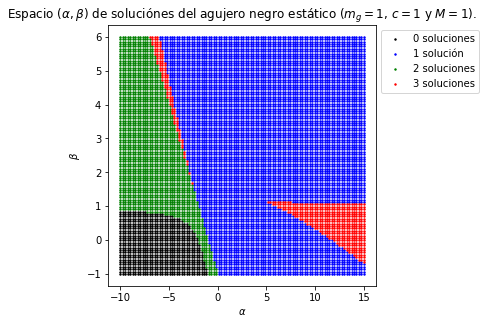
\includegraphics[scale=0.45]{SoluciónEstática/Horizonte de Eventos/HorizonsNum1.png}
         \caption{Soluciones en el espacio $(\alpha-\beta)$ con $M=1$.}
         \label{fig:M1}
     \end{subfigure}
     \hspace{1cm}
     \begin{subfigure}[b]{0.4\textwidth}
         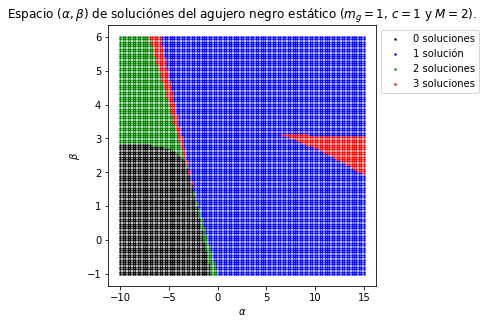
\includegraphics[scale=0.45]{SoluciónEstática/Horizonte de Eventos/HorizonsNum2.png}
         \caption{Soluciones en el espacio $(\alpha-\beta)$ con $M=2$.}
         \label{fig:M2}
     \end{subfigure}    
      \hfill
      \begin{subfigure}[b]{0.4\textwidth}
          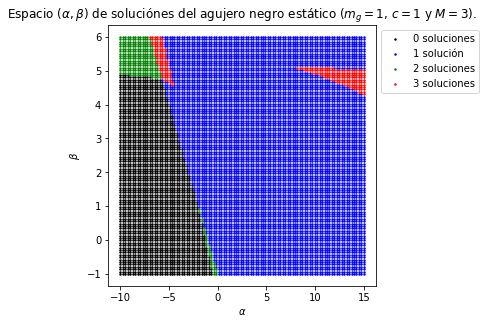
\includegraphics[scale=0.45]{SoluciónEstática/Horizonte de Eventos/HorizonsNum3.png}
          \caption{Soluciones en el espacio $(\alpha-\beta)$ con $M=3$.}
          \label{fig:M3}
      \end{subfigure}
    \hspace{1cm}
    \begin{subfigure}[b]{0.4\textwidth}
    \centering
        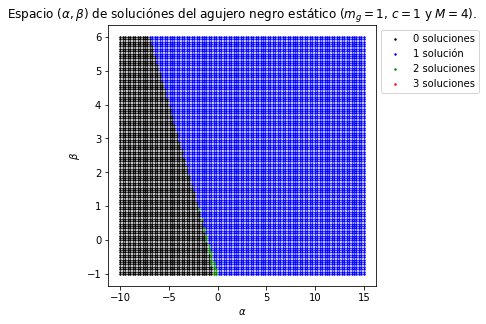
\includegraphics[scale=0.45]{SoluciónEstática/Horizonte de Eventos/HorizonsNum4.png}
        \caption{Soluciones en el espacio $(\alpha-\beta)$ con $M=4$.}
        \label{fig:M4}
    \end{subfigure}
     
     \caption{Número de soluciones a la ecuación \eqref{eq:solucionesHorizonte} en el espacio $(\alpha-\beta)$ con $m_g=1$ y $\epsilon=1$ para distintos valores de $M$. }
     \label{fig:NumHorizon}
 \end{figure}
 
 En todas las gráficas de la figura \ref{fig:NumHorizon} hay una clara diferenciación entre la región de numero de soluciones pares y número de soluciones impares, la linea recta que divide estas regiones coincide con $\Lambda=-3m_g^2(1+\alpha+\beta)=0$, lo cual coincide con lo esperado. En la región donde se encuentra un número par de soluciones, corresponde a la región $\Lambda>0$  que para la forma de la solución \eqref{eq:StaticF} corresponde al espacio de de Sitter (dS) \cite{AClassOfBlackHoles}. Mientras que en la región donde se encuentra un número impar de soluciones corresponde a el espacio $\Lambda<0$ que corresponde al espacio anti de Sitter (AdS) \cite{AClassOfBlackHoles}. Adicionalmente, mientras los valores de la masa del agujero negro $M$ aumentan las regiones que tienen mayor peso son las de una o cero soluciones, tendiendo a la cantidad de soluciones de Schwarzschild.\\

 
 \begin{figure}[H]
     \centering
     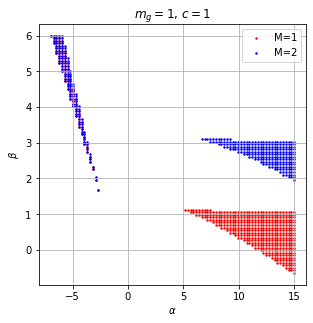
\includegraphics[scale=0.45]{SoluciónEstática/Horizonte de Eventos/Artículo.png}
     \caption{Región en el espacio $(\alpha-\beta)$ con $m_g=1$, $\epsilon=1$ y $M=1$ ($M=2$), para la región roja (azul), con tres horizontes de eventos.}
     \label{fig:articleHorizons}
 \end{figure}
 
   Superponiendo las regiones con tres soluciones de horizontes de eventos con $M=1$ y $M=2$ se obtiene la figura \ref{fig:articleHorizons}, la cual reproduce los resultados obtenidos en \cite{AClassOfBlackHoles}. En la figura \ref{fig:articleHorizons} la región superior izquierda corresponde a una región compartida por los dos valores de masa, mientras que las otras regiones se distinguen fácilmente.\\
 
   La comparativa de la forma de la función \eqref{eq:StaticF} respecto de la solución de Schwarzschild se muestra en la figura \ref{fig:F(r)sols}, donde se pueden comparar la forma para cada número posible de soluciones, donde la figura \ref{fig:F(R)sols2} presentan horizonte cosmológico, como es de esperarse para el espacio dS. Mientras que las figuras \ref{fig:F(R)sols1} y \ref{fig:F(R)sols3} presentan sólo horizonte de eventos, aspecto que nuevamente es esperable al pertenecer al espacio AdS. Cada uno de los valores de $\alpha$ y $\beta$ fueron escogidos según las regiones de la figura \ref{fig:F(r)sols}), esto también permite comprobar los resultados de esta misma figura.\\
 \begin{figure}[H]
    \centering
    \ContinuedFloat*
     \begin{subfigure}[b]{0.4\textwidth}
         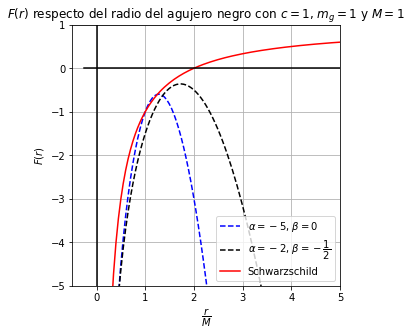
\includegraphics[scale=0.45]{SoluciónEstática/Horizonte de Eventos/F(r) Estática0.png}
         \caption{Gráfica de la ecuación \eqref{eq:StaticF} con ningún horizonte de eventos.}
         \label{fig:F(R)sols0}
     \end{subfigure}
     \hspace{1cm}
     \begin{subfigure}[b]{0.4\textwidth}
         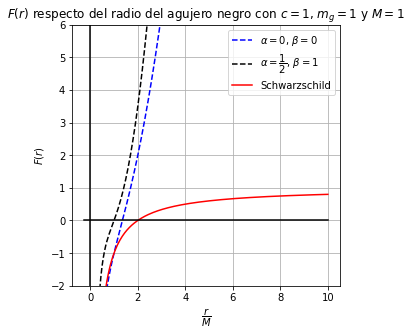
\includegraphics[scale=0.45]{SoluciónEstática/Horizonte de Eventos/F(r) Estática1.png}
         \caption{Gráfica de la ecuación \eqref{eq:StaticF} con un horizonte de eventos.}
         \label{fig:F(R)sols1}
     \end{subfigure} 
\end{figure}
\begin{figure}[H]
\ContinuedFloat
      \hfill
      \begin{subfigure}[b]{0.4\textwidth}
          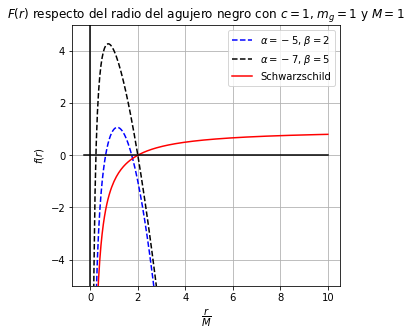
\includegraphics[scale=0.45]{SoluciónEstática/Horizonte de Eventos/F(r) Estática2.png}
          \caption{Gráfica de la ecuación \eqref{eq:StaticF} con dos horizontes de eventos.}
          \label{fig:F(R)sols2}
      \end{subfigure}
    \hspace{1cm}
    \begin{subfigure}[b]{0.4\textwidth}
    \centering
        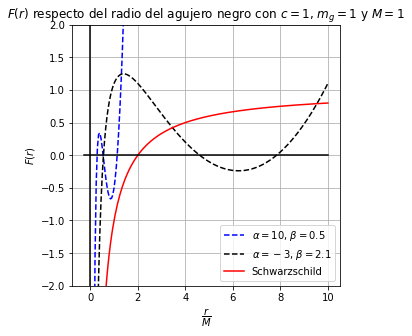
\includegraphics[scale=0.45]{SoluciónEstática/Horizonte de Eventos/F(r) Estática3.png}
        \caption{Gráfica de la ecuación \eqref{eq:StaticF} con tres horizontes de eventos.}
        \label{fig:F(R)sols3}
    \end{subfigure}
     
     \caption{Gráfica de la ecuación \eqref{eq:StaticF} con $\epsilon=1$, $m_g=1$ y $M=1$ para distintos valores de $\alpha$ y $\beta$.}
     \label{fig:F(r)sols}
 \end{figure}
  
  La gráfica roja en cada gráfica de la figura \ref{fig:F(r)sols} corresponde a la ecuación \eqref{eq:StaticF} con $m_g=0$ y $M=1$ que corresponde a la solución de Schwarzschild. Adicionalmente la figura \ref{fig:F(R)sols3} corresponde a los valores de $\alpha$ y $\beta$ usados en \cite{AClassOfBlackHoles}, donde, nuevamente, se reproducen los resultados registrados allí.\\
  
  Una de las cualidades del universo posible dada la función $F(r)$ son las regiones donde $F(r)>0$, regiones donde la métrica se comporta de la manera esperada. En la figura \ref{fig:F(r)sols} las gráficas que cumplen con condiciones esperadas de $F(r)>0$ son las figuras \ref{fig:F(R)sols1} y \ref{fig:F(R)sols3}, mientras que la figura \ref{fig:F(R)sols0} presenta singularidad desnuda y la figura \ref{fig:F(R)sols2} presenta problemas en la métrica debido a $F(r)<0$, las soluciones en estas regiones son descartables para la mayoría de valores de $\alpha $ y $\beta$.\\
 
  
  Todas las gráficas mostradas anteriormente y su implementación pueden ser encontradas con mayor detalle en \cite{GitHub}.

\section{Termodinámica de la solución estática} 

Otra característica que resulta de interés en algunas ocasiones es el estudio del comportamiento termodinámico del agujero negro. En especial, la gravedad superficial $\kappa$, la cual está relacionada con la temperatura y la entropía. Para la solución estática de agujero negro, se asumirá que el agujero negro es un sistema aislado, es decir, no hay ningún tipo transferencia de partículas, ni creación ni aniquilación \cite{AClassOfBlackHoles}.

\subsection{Gravedad superficial}

Usando la ecuación \eqref{eq:HorizonEq} del horizonte de eventos se encuentra que la masa del agujero negro en términos del horizonte de eventos $r_+$ viene dada por

\begin{equation}
    M=\dfrac{r_+}{2}\left(1-\dfrac{\Lambda}{3}r_+^2+\gamma r_++\zeta\right),
\end{equation}

usando los valores de las ecuaciones \eqref{eq:Lambda}, \eqref{eq:gamma} y \eqref{eq:zeta}, usando que $m_g=\epsilon=1$ por simplicidad y reordenando los términos se obtiene que

\begin{equation}
    M=\dfrac{r_+}{2}\left(\alpha(r_+-1)^2+\beta(r_+^2-3r_++3)+r_+^2-r_++1\right).
    \label{eq:MassAlphaBetaStatic}
\end{equation}

Las condiciones para obtener un agujero negro con masa negativa son

\begin{gather}
    \alpha>-\dfrac{\beta(r_+^2-3r_++3)+r_+^2-r_++1}{(r_+-1)^2}, \text{ para } r_+\neq 1\\
    \beta > -1 \text{ para cualquier valor de $\alpha$ y } r_+=1.
\end{gather}

Por otro lado, la gravedad superficial $\kappa$ para un agujero negro esféricamente simétrico y estático viene dada por la expresión $\kappa=\dfrac{F'(r_+)}{2}$ donde $F'(r)$ corresponde a la derivada total de la función $F$ \cite{ToolKit}, en esta caso de \eqref{eq:StaticF}, por tanto la gravedad superficial viene dada por

\begin{equation}
    \kappa=\dfrac{1}{2}\left(\dfrac{2M}{r_+^2}-\dfrac{2\Lambda}{3} r_+ + \gamma\right),
\end{equation}

usando la ecuación \eqref{eq:MassAlphaBetaStatic}, se llega a

\begin{equation}
    \kappa=\dfrac{1}{2r_+}\left(1-\Lambda r_+^2+2\gamma r_++\zeta\right).
    \label{eq:StaticSurfaceGravity}
\end{equation}

Dado que la gravedad superficial no depende de ningún parámetro además de $r_+$ esta es constante en todo el horizonte de eventos, es decir, se cumple la ley cero de la termodinámica de agujeros negros.

\subsubsection{Temperatura}

En general, para cualquier agujero negro se cumple que 

\begin{equation}
    T=\dfrac{\kappa}{2\pi},
\end{equation}

con $\kappa$ la gravedad superficial, usando la ecuación \eqref{eq:StaticSurfaceGravity} se obtiene entonces

\begin{equation}
    T=\dfrac{1}{4\pi r_+}\left(1-\Lambda r_+^2+2\gamma r_++\zeta\right).
    \label{eq:StaticTemperature}
\end{equation}

Tomando el límite $m_g\rightarrow 0$ se tiene $T=\dfrac{1}{4\pi r_+}$, recuperando la temperatura para el agujero negro de Schwarzschild.\\ 

Debido a la forma de la temperatura esta presenta un mínimo local $T_{(min)}$, a través del cual se puede asegurar la condición de $T>0$. Derivando la ecuación \eqref{eq:StaticTemperature} y encontrando el valor de $r_+$ para el cual se tiene $T_{(min)}$, se encuentra que

\begin{equation}
    r_{+(min)}=\sqrt{-\dfrac{1+\zeta}{\Lambda}}=\sqrt{\dfrac{1+\alpha+3\beta}{3(1+\alpha+\beta)}}.
    \label{eq:rMin}
\end{equation}

Reemplazando el valor de $r_+$ por el valor de la ecuación \eqref{eq:rMin}, se obtiene el valor mínimo de la temperatura, la cual dependería del valor de $\alpha$ y $\beta$, esta queda escrita como sigue

\begin{equation}
    T_{(min)}=\dfrac{1}{2\pi}\sqrt{-\dfrac{\Lambda}{1+\zeta}}\left(1+\zeta+2\gamma\sqrt{-\dfrac{1+\zeta}{\Lambda}}\right)
\end{equation}

Dado que la temperatura mínima $T_{(min)}$ se escribe en términos de $\alpha$ y $\beta$ es posible realizar un gráfico de las regiones donde esta es $T_{(min)}>0$ y a la vez se cumple que $r_{(min)>0}$, la gráfica \ref{fig:TemperaturaStatic} muestra las regiones para estos valores, para la cual existe una región donde la temperatura es mayor que cero en todo punto de $r>0$. Además, la región está contenida en la región donde $r_{(min)}>0$.

\begin{figure}[H]
    \centering
    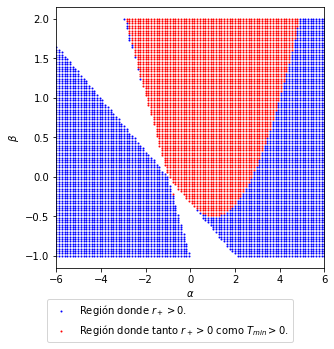
\includegraphics[scale = 0.5]{SoluciónEstática/Termodinámica/Temperatura.png}
    \caption{Región del espacio $(\alpha-\beta)$ en el cual $T_{(min)}>0$, en rojo y $r_{(min)}>0$, en azul. La gráfica fue generada usando el código disponible en \cite{GitHub}.}
    \label{fig:TemperaturaStatic}
\end{figure}

A pesar de que la temperatura existe para algunos valores de $r_{(min)}>0$ estos valores también deben estar contenidos en las regiones donde hay soluciones válidas. En la figura \ref{fig:StaticTempAlphayBeta} se tiene la región roja de la figura \ref{fig:TemperaturaStatic} sobre las regiones de la gráfica \ref{fig:M1}, en esta gráfica se encuentra que la región donde $T$ es completamente positiva corresponde a la región donde hay solo una solución, esto para el caso de $M=m_g=\epsilon=1$, valores en los cuales la métrica tiene un comportamiento esperado.

\begin{figure}[H]
   \centering
    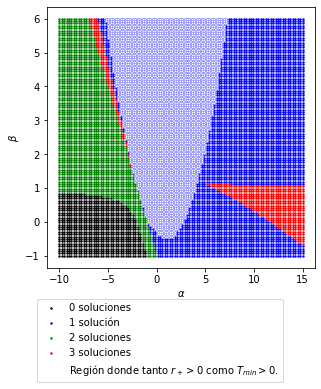
\includegraphics[scale = 0.5]{SoluciónEstática/Termodinámica/Temperatura_alphaBeta.png}
    \caption{Región donde $T_{(min)}>0$ y $r_{(min)}>0$, en blanco, sobre la región donde hay soluciones de agujero negro según la figura \ref{fig:M1}. La gráfica y el código que la genera está disponible en \cite{GitHub}.}
    \label{fig:StaticTempAlphayBeta}
\end{figure}

Para corroborar los resultados de las figuras \ref{fig:TemperaturaStatic} se graficó el comportamiento de la temperatura en función de $r$ para valores de las dos diferentes regiones, estos resultados se ven en la gráfica \ref{fig:T(r)Static}. La gráfica \ref{fig:T(r)static0} es la temperatura para valores de $\alpha$ y $\beta$ donde $T>0$ t $r_{(min)}>0$, mientras que en \ref{fig:T(r)static1} es la gráfica de la temperatura donde $r_{(min)}>0$ pero no necesariamente $T>0$.

\begin{figure}[H]
    \centering
    \begin{subfigure}[b]{0.4\textwidth}
         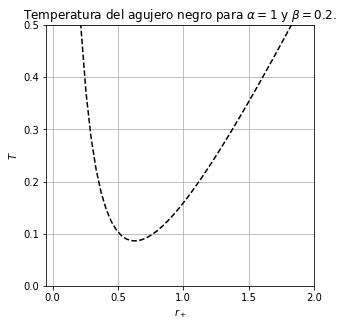
\includegraphics[scale=0.5]{SoluciónEstática/Termodinámica/T(R)0.png}
         \caption{Temperatura en términos de $r$ donde $T>0$, para todo $r>0$.}
         \label{fig:T(r)static0}
     \end{subfigure}
     \begin{subfigure}[b]{0.4\textwidth}
         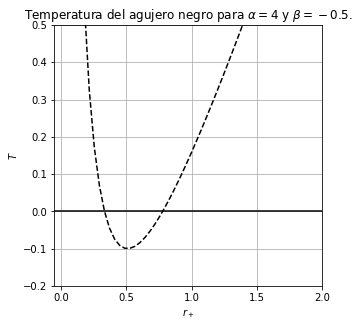
\includegraphics[scale=0.5]{SoluciónEstática/Termodinámica/T(r)1.png}
         \caption{Temperatura en términos de $r$ donde el agujero negro se congela.}
         \label{fig:T(r)static1}
     \end{subfigure}
    \label{fig:T(r)Static}
    \caption{Comportamiento de la temperatura para distintos valores en la región $(\alpha-\beta)$.}
\end{figure}

Si bien es esperable que tener un comportamiento de $T>0$ no sea problemático, en el caso del comportamiento de la ecuación \eqref{eq:StaticTemperature} presenta el mismo problema de la evaporación del agujero negro de Schwarzschild y la perdida de la información, sin embargo, las regiones donde $T_{(min)}$ es menor a cero, el agujero negro se congela y conserva la información al interior del horizonte de eventos.

\subsection{Entropía}

Para el caso de la entropía, esta se puede encontrar a través de la primera ley de la termodinámica de agujeros negros \cite{ToolKit, AClassOfBlackHoles} $dM=TdS$, es decir,

\begin{equation}
    S=\int \dfrac{dM}{T}=\int \dfrac{1}{T}\dfrac{\partial M}{\partial r_+}dr_+.
\end{equation}

Dado que $\dfrac{\partial M}{\partial r_+}=2\pi r_+T$, se obtiene que la entropía del agujero negro será 

\begin{equation}
    S=\pi r_+^2=\dfrac{A_+}{4},
\end{equation}

con $A_+$ el área superficial del agujero negro, encontrando que a pesar de introducir el potencial de la teoría dRGT la entropía no se ve afectada, es decir, la entropía corresponde al caso de Schwarzschild. 

%\section{Órbita ISCO y esféra de fotónes} 
\chapter{Solución rotante}
\label{chap:Rotante}

Si bien la solución estudiada en el capítulo \ref{chap:staticSolution} es una solución que resuelve las ecuaciones de campo de la ecuación \eqref{eq:fieldEquations}, esta solución es una solución estática cuyo tensor momento energía $T_{\mu\nu}=0$. Una de las soluciones de las ecuaciones de campo de la relatividad General ($m_g=0$) es la solución de agujero negro tipo Kerr, esta solución corresponde a un agujero negro con masa que además gira.\\

La solución de tipo Kerr, es una solución que es mucho más compleja comparada con la solución de Schwarzschild, es por ello que se han estudiado maneras de generar la solución de alguna manera \cite{JN-RotatingAndNUTCharged}. Uno de los algoritmos que han probado servir para generar soluciones rotantes es el algoritmo de Janis Newman, a través del cual se generó la solución rotante de Kerr, a partir de la solución de Schwarszchild \cite{JN-RotatingAndNUTCharged}.

\section{Algoritmo de Janis-Newman}

El algoritmo de Janis-Newman es una de las técnicas para generar métricas rotantes a través de métricas estáticas \cite{JN-RotatingAndNUTCharged}. Si bien en un principio se postuló como un algoritmo para generar soluciones en relatividad general, pues se ha considerado como una derivación alternativa de la métrica de Kerr que posteriormente se usó para obtener el agujero negro de Kerr-Newman \cite{JN-RotatingAndNUTCharged, AnExtensionOfJN}, esta ha funcionado al aplicarse en otras teorías \cite{JN-RotatingAndNUTCharged}.\\

El algoritmo puede resumirse como sigue \cite{JN-RotatingAndNUTCharged, AnExtensionOfJN}: 

\begin{enumerate}
    \item Determinar la métrica denominada como  "semilla", y usar las coordenadas de Eddington-Finkelstein, haciendo una transformación de $(t,r,\theta,\phi)$ a $(u,r,\theta\phi)$.
    \item Realizar una transformación compleja de coordenadas a la estructura tensorial $dx^\mu$ y la función $f$. La transformación de coordenadas puede ser realizada usando el formalismo de tetradas de Newman-Penrose.
    \item Realizar una transformación de coordenadas para simplificar la métrica, como puede ser el sistema de coordenadas de Boyer-Lindquist.
\end{enumerate}

\subsection{Janis-Newman: Formalismo de Newman-Penrose}

Una de las formas de llevar a cabo el algoritmo de Janis-Newman es usando el formalismo de Newman-Penrose de tetradas. El formalismo de Newman-Penrose consiste en la escogencia de un una base coordenada especial, llamada una base nula \cite{ThePotentialOfFildsInEinstein}.\\

En lugar de una base ortogonal, Newman y Penrose escogieron una base nula con un par de tensores reales $l^\mu$, $n^\mu$ y un par de tensores conjugados $m^\mu$ y $\bar{m}^\mu$ tal que

\begin{gather}
    l^\mu m_\mu = l^\mu \bar{m}_\mu = n^\mu m_\mu = n^\mu \bar{m}_\mu = 0, \label{eq:Nulity0}\\
    l^\mu l_\mu = n^\mu n_\mu = m^\mu m_\mu = \bar{m}^\mu\bar{m}_\mu = 0, \label{eq:Nulity1}
\end{gather}

junto con la condición de normalización 

\begin{equation}
    -l^\mu n_\mu = m^\mu \bar{m}_\mu = 1,
    \label{eq:Unitarity}
\end{equation}

lo anterior implica que la matriz que transforma en el espacio de las tetradas viene dada por

\begin{equation}
    [\eta_{(a)(b)}]=\begin{pmatrix}
        0 & -1 & 0 & 0 \\
        -1 & 0 & 0 & 0 \\
        0 & 0 & 0 & 1 \\
        0 & 0 & 1 & 0 \\
    \end{pmatrix}.
\end{equation}

Luego, la métrica $g^{\mu\nu}$ puede ser escrita en términos de los tensores $(l^\mu,n^\mu,m^\mu,\bar{m}^\mu)$ como sigue \cite{ThePotentialOfFildsInEinstein}

\begin{equation}
    g^{\mu\nu}=-l^\mu n^\nu-l^\nu n^\mu+m^\mu \bar{m}^\nu+m^\nu \bar{m}^\mu.
    \label{eq:TetradMetric}
\end{equation}

Al realizar la transformación de coordenadas $x^\mu\rightarrow \tilde{x}^\mu$ cada uno de los tensores $(l^\mu,n^\mu,m^\mu,\bar{m}^\mu)$ transforman como 
\begin{equation}
    \tilde{Z}^\mu=\dfrac{\partial \tilde{x}^\mu}{\partial x^\nu}Z^\nu,
    \label{eq:tetradTransformation}
\end{equation}

donde la nueva métrica $\tilde{g}$ vendrá dada por

\begin{equation}
    \tilde{g}^{\mu\nu}=-\tilde{l}^\mu \tilde{n}^\nu-\tilde{l}^\nu \tilde{n}^\mu+\tilde{m}^\mu \tilde{\bar{m}}^\nu+\tilde{m}^\nu \tilde{\bar{m}}^\mu.
    \label{eq:TetradMetricComplex}
\end{equation}

Con lo anterior, es posible usar la métrica que describe el elemento de línea de la ecuación \eqref{eq:staticSolution} para obtener una métrica rotante en la gravedad dRGT.

\section{Agujero negro rotante}

\subsection{Paso 1: Métrica semilla en coordenadas Eddington-Finkelstein}
    Como se comentó anteriormente, el paso 1 del algoritmo consiste en seleccionar una métrica "semilla" sobre la cual se aplicará el algoritmo. Esta métrica semilla es la métrica que describe el elemento de línea de la ecuación \eqref{eq:staticSolution} con $F(r)$ descrito en \eqref{eq:StaticF}.\\
    
    Para obtener la ecuación \eqref{eq:staticSolution} en las coordenadas de Enddington-Finkelstein se realiza el siguiente cambio de coordenadas
    \begin{equation}
        dt=du-\dfrac{dr}{F(r)},
    \end{equation}
    
    con lo cual el elemento de línea queda escrito como
    
    \begin{equation}
        ds^2=-F(r)du^2+2dudr+r^2d\Omega^2.
        \label{eq:seedMetricEF}
    \end{equation}
    
    Con lo cual la métrica $g_{\mu\nu}$ queda descrita, en su representación matricial, como sigue
    
    \begin{equation}
        [g_{\mu\nu}]=\begin{pmatrix}
            -F & 1 & 0   & 0 \\
             1 & 0 & 0   & 0 \\
             0 & 0 & r^2 & 0\\
             0 & 0 & 0 & r^2\sin^2\theta
        \end{pmatrix},
    \end{equation}
    
    mientras que la métrica en su forma contravariante vendrá dada como sigue
    
    \begin{equation}
        [g^{\mu\nu}]=\begin{pmatrix}
             0 & 1 & 0   & 0 \\
             1 & F & 0   & 0 \\
             0 & 0 & \dfrac{1}{r^2} & 0\\
             0 & 0 & 0 & \dfrac{1}{r^2\sin^2\theta}
        \end{pmatrix}.
    \end{equation}
    
\subsection{Paso 2: Formalismo de Newman-Penrose y transformación compleja de la función semilla $F(r)$}

Para realizar la transformación compleja de la métrica es necesario realizar una correcta selección de las tetradas de Newman-Penrose, las tetradas quedan definidas como sigue \cite{AplicabilityOfJN}

\begin{gather}
    l^\mu = \delta^\mu_r, \\
    n^\mu = \delta^\mu_u-\delta^\mu_r\dfrac{F}{2}, \\
    m^\mu = \dfrac{1}{\sqrt{2}r}\left(\delta^\mu_\theta+ \dfrac{i}{\sin \theta}\delta^\mu_\phi\right),
\end{gather}

las cuales cumplen con las condiciones \eqref{eq:Nulity0}, \eqref{eq:Nulity1} y \eqref{eq:Unitarity}, además que también describe la métrica según la ecuación \eqref{eq:TetradMetric}.\\

Tras definir las tetradas las coordenadas $u$ y $r$ puede tomar valores complejos, pero manteniendo que $l^\mu$ y $n^\mu$ reales, junto con $(m^\mu)^*=\bar{m}^\mu$ y reemplazando $F(r)\rightarrow \tilde{F}(r,\tilde{r})$, luego se realiza la siguiente transformación sobre las coordenadas \cite{AplicabilityOfJN},

\begin{equation}
    x^\mu\rightarrow\tilde{x}^\mu=x^\mu+ia\cos\theta(\delta^\mu_{\tilde{u}}-\delta^\mu_{\tilde{r}}),
\end{equation}

donde $a$ será identificada más adelante como el parámetro de espín.\\

Usando la transformación de tetradas descrita por \eqref{eq:tetradTransformation}, se tienen las nuevas tetradas, escritas como sigue \cite{AplicabilityOfJN}

\begin{gather}
    \tilde{l}^\mu = \delta^\mu_r,\\
    \tilde{n}^\mu = -\delta^\mu_u-\dfrac{1}{2}\tilde{F}(r,\tilde{r})\delta^\mu_r,\\
    \tilde{m}^\mu = \dfrac{1}{\sqrt{2}(r+ia\cos\theta)}\left(ia\sin\theta\left(\delta^\mu_r+\delta^\mu_u\right)+\delta^\mu_\theta+\dfrac{i}{\sin\theta}\delta^\mu_\phi\right).
\end{gather}

Definiendo $\rho$ como 
\begin{equation}
    \rho^2 = |\tilde{r}|^2 = (r+ia\cos\theta)(r-ia\cos\theta)=r^2+a^2\cos^2\theta,
\end{equation}

y usando la ecuación \eqref{eq:TetradMetricComplex}, se obtienen los siguientes términos para la métrica $\tilde{g}^{\mu\nu}$

\begin{equation}
    [g^{\mu\nu}]=
    \begin{pmatrix}
        \dfrac{a^2\sin^2\theta}{\rho^2} & 1+ \dfrac{a^2\sin^2\theta}{\rho^2} &   0 &     \dfrac{a}{\rho^2}\\
        1+ \dfrac{a^2\sin^2\theta}{\rho^2} &    \tilde{F}+\dfrac{a^2\sin^2\theta}{\rho^2} &   0 &   \dfrac{\alpha}{\rho^2}\\
        0 &    0&   \dfrac{1}{\rho^2} &  0\\
         \dfrac{a}{\rho^2}    & \dfrac{\alpha}{\rho^2}   &   0&   \dfrac{1}{\rho^2\sin^2\theta} \\
    \end{pmatrix}
    \label{eq:MetricaRotanteContravariante}
\end{equation}

Uno de los aspectos menos comprendidos sobre el algoritmo es la forma de realizar la transformación compleja de la función $F(r)$ de la semilla \cite{AnExtensionOfJN, JN-RotatingAndNUTCharged}. Si bien esta transformación es arbitraria se han cubierto diferentes transformaciones complejas, una transformación que ha funcionado para no solo el caso de Kerr, sino también para soluciones de tipo dS y AdS.\\

La transformación de la función $F(r)$ va como sigue,

\begin{equation}
    \tilde{F}(r,\tilde{r})=1-\dfrac{2m(r)}{r}\left(\dfrac{r^2}{\rho^2}\right),
\end{equation}

donde $m(r)$ es la función de masa de la función raíz $F(r)$ como una función de r. Con los elementos obtenidos anteriormente, resta encontrar la métrica en su forma covariante ($\tilde{g}_{\mu\nu}$) y reescribirla en coordenadas Boyer-Lindquist.

\subsection{Paso 3: Reescribir la métrica en coordenadas de Boyer-Lindquist}

La métrica en su forma covariante es el tensor $g_{\mu\nu}$ tal que $g^{\mu\nu}g_{\mu\nu}=\mathbb{I}$, en términos de la representación matricial es la matríz inversa de la ecuación \eqref{eq:MetricaRotanteContravariante}. Por tanto, el tensor $g_{\mu\nu}$ viene dado por

\begin{equation}
    [g_{\mu\nu}]=\begin{pmatrix}- \tilde{F} & 1 & 0 & a \left(\tilde{F} - 1\right) \sin^{2}{\theta}\\1 & 0 & 0 & - a \sin^{2}{\theta}\\0 & 0 & \rho^{2} & 0\\a \left(\tilde{F} - 1\right) \sin^{2}{\theta} & - a \sin^{2}{\theta} & 0 & \left(\rho^{2} + (2-\tilde{F}) a^{2} \sin^{2}{\theta}\right) \sin^{2}{\theta}\end{pmatrix},
\end{equation}

o escrito en términos del elemento de línea queda como

\begin{equation}
    \begin{split}
    d\tilde{s}^2=-\tilde{F}du^2+2dudr+\rho^2d\theta^2+\left(\rho^{2} + (\tilde{F}-2) a^{2} \sin^{2}{\theta}\right) \sin^{2}{\theta}d\phi^2\\
    +2a \left(\tilde{F} - 1\right) \sin^{2}{\theta}dud\phi-2a\sin^2\theta (\tilde{F}-2) drd\phi
    \label{eq:LineElementRotating}
\end{split}
\end{equation}

Para realizar la transformación a coordenadas en Boyer-Lindquist es necesario realizar los siguientes cambios sobre los diferenciales \cite{AplicabilityOfJN}

\begin{gather}
    du = dt+g(r)dr, \label{eq:du}\\
    d\phi = d\phi+h(r)dr \label{eq:dphi},
\end{gather}

con $g(r)$ y $h(r)$ funciones ajustadas de tal manera que $g_{r\phi}=g_{tr}=0$. Reemplazando los diferenciales en \eqref{eq:du} y \eqref{eq:dphi} en la ecuación \eqref{eq:LineElementRotating} se obtiene que las funciones $g$ y $h$ deben ser como sigue 

\begin{gather}
    g(r) =  \dfrac{r^2+a^2}{\Delta}, \label{eq:gJN}\\
    h(r) =  \dfrac{a}{\Delta}. \label{eq:hJN}
\end{gather}

con 

\begin{equation}
    \Delta = \rho^2\tilde{F}+a^2\sin^2\theta.
\end{equation}

Luego, usando las ecuaciones \eqref{eq:gJN} y \eqref{eq:hJN} se obtiene el siguiente elemento de línea para la solución rotante

\begin{equation}
        d\tilde{s}^2= -\tilde{F}dt^2+\dfrac{\rho^2}{\Delta}dr^2+\rho^2d\theta^2+(\rho^2+(\tilde{F}-2)a^2\sin^2\theta)\sin^2\theta d\phi^2 + 2a\sin^2\theta d\phi dt.
        \label{eq:tildeElementoDeLinea}
\end{equation}

La representación matricial de la métrica resultante para la solución rotante vendrá expresada como

\begin{equation}
    [\tilde{g}_{\mu\nu}]=
    \begin{pmatrix}
        -\tilde{F}& 0 & 0 & (F-1)a\sin^2\theta\\
        0&  \dfrac{\rho^2}{\Delta}& 0&  0 \\
        0&  0&  \rho^2& 0\\
        (F-1)a\sin^2\theta&  0&  0&  (\rho^2+(\tilde{F}-2)a^2\sin^2\theta)\sin^2\theta\\  \label{eq:TildeMétrica}
    \end{pmatrix}.
\end{equation}

\section{Métrica de la solución rotante}

Se aplicó el algoritmo de Janis Newman a la solución estática de la ecuación \eqref{eq:staticSolution}, donde la función semilla viene dada por la ecuación \eqref{eq:StaticF}. Para el caso de la solución \eqref{eq:StaticF} se tiene que

\begin{equation}
    m(r)=M+\dfrac{\Lambda}{6}r^3-\dfrac{\gamma}{2}r^2-\dfrac{\zeta}{2}r.
\end{equation}

Por tanto, $\tilde{F}(r,\tilde{r})$ viene dada por

\begin{equation}
    \tilde{F}(r,\tilde{r})=1-\dfrac{1}{\rho^2}\left(2Mr+\dfrac{\Lambda}{3}r^4-\gamma r^3-\zeta r^2\right).
    \label{eq:FTilde}
\end{equation}

Reemplazando la ecuación \eqref{eq:FTilde} en \eqref{eq:tildeElementoDeLinea} se obtiene el elemento de linea para el agujero negro rotante en gravedad dRGT, el cual viene dado como sigue

\begin{equation}
\begin{split}
    d\tilde{s}^2= -\left(1-\dfrac{1}{\rho^2}\left(2Mr+\dfrac{\Lambda}{3}r^4-\gamma r^3-\zeta r^2\right)\right)dt^2+\dfrac{\rho^2}{\Delta}dr^2+\rho^2d\theta^2\\
    +\left[\rho^2-\left(1+\dfrac{1}{\rho^2}\left(2Mr+\dfrac{\Lambda}{3}r^4-\gamma r^3-\zeta r^2\right)\right)a^2\sin^2\theta\right]\sin^2\theta d\phi^2\\
    -\dfrac{2a\sin^2\theta}{\rho^2}\left(2Mr+\dfrac{\Lambda}{3}r^4-\gamma r^3-\zeta r^2\right) d\phi dt,
\end{split}
        \label{eq:ElementoDeLineaSolucionRotante}
\end{equation}

donde $\Delta = \rho^2 - 2Mr - \dfrac{\Lambda}{3}r^4+\gamma r^3+\zeta r^2+a^2\sin^2\theta$, usando la definición de $\rho^2$, se obtiene la siguiente expresión para $\Delta$


\begin{equation}
    \Delta = -\dfrac{\Lambda}{3}r^4+\gamma r^3 + (\zeta+1)r^2
\end{equation}


Para el elemento de linea mostrado en la ecuación \eqref{eq:ElementoDeLineaSolucionRotante} es posible corroborar que cuando el parámetro de espín del agujero negro $a$ tiende a cero, se recupera el elemento de linea de la solución estática, es decir, \eqref{eq:staticSolution} con $F(r)$ definido en \eqref{eq:StaticF}.

\section{Horizonte de eventos}


\section{Ergosfera}


\section{Gravedad superficial}
\chapter{Cap\'{\i}tulo ...}
Se deben incluir tantos cap\'{\i}tulos como se requieran; sin embargo, se recomienda que la tesis  o trabajo de investigaci\'{o}n tenga un m\'{\i}nimo 3 cap\'{\i}tulos y m\'{a}ximo de 6 cap\'{\i}tulos (incluyendo las conclusiones).\\
\chapter{Conclusiones}
\label{chap:Conclusiones}
\section{Conclusiones}
Las conclusiones constituyen un cap\'{\i}tulo independiente y presentan, en forma l\'{o}gica, los resultados de la tesis  o trabajo de investigaci\'{o}n. Las conclusiones deben ser la respuesta a los objetivos o prop\'{o}sitos planteados. Se deben titular con la palabra conclusiones en el mismo formato de los t\'{\i}tulos de los cap\'{\i}tulos anteriores (T\'{\i}tulos primer nivel), precedida por el numeral correspondiente (seg\'{u}n la presente plantilla).\\

\section{Recomendaciones}
Se presentan como una serie de aspectos que se podr\'{\i}an realizar en un futuro para emprender investigaciones similares o fortalecer la investigaci\'{o}n realizada. Deben contemplar las perspectivas de la investigaci\'{o}n, las cuales son sugerencias, proyecciones o alternativas que se presentan para modificar, cambiar o incidir sobre una situaci\'{o}n espec\'{\i}fica o una problem\'{a}tica encontrada. Pueden presentarse como un texto con caracter\'{\i}sticas argumentativas, resultado de una reflexi\'{o}n acerca de la tesis o trabajo de investigaci\'{o}n.\\
\begin{appendix}
\chapter{Anexo: Formalismo de Newman-Penrose y algorítmo de Janis Newman}\label{AnexoA}




\end{appendix}
\addcontentsline{toc}{chapter}{\numberline{}Bibliograf\'{\i}a}
\bibliographystyle{unsrtnat}
\bibliography{Referencias}
\end{document}